\subsection{Modello E-R}
Per la realizzazione del modello entità-relazione si è deciso di seguire una strategia mista, isolando l'attività della base di dati in 3 parti principali. 
\begin{itemize}
    \item La prima parte verterà sull'entità Cliente: la creazione di un ordine e la scrittura di una recensione.
    
    \item La seconda parte si concentrerà sull'entità Prodotto: l'appartenenza ad una specifica categoria e la sua variazione di prezzo in caso di sconto.
    
    \item La terza parte tratterà l'entità Segnalazione e ciò che comporta la risoluzione della stessa.
\end{itemize}In seguito sarà possibile unire le tre macro-parti nuove relazioni tra entità implicate. Ci si pone come obbiettivo la realizzazione di un modello privo di ridondanze e già normalizzato. 

\subsubsection{Cliente}
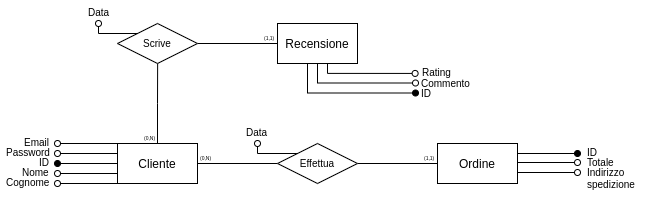
\includegraphics[scale=0.65]{images/cliente.png}
\textbf{Si è scelto di identificare l'entità Cliente attraverso un ID numerico} invece che con\textbf{ l'attributo email}, anche se questa \textbf{rimane altresì una chiave candidata}, \textit{per la quale vige vincolo di univocità}; in questo modo si favorisce la pseudonimizzazione dei dati.

\subsubsection{Prodotto}
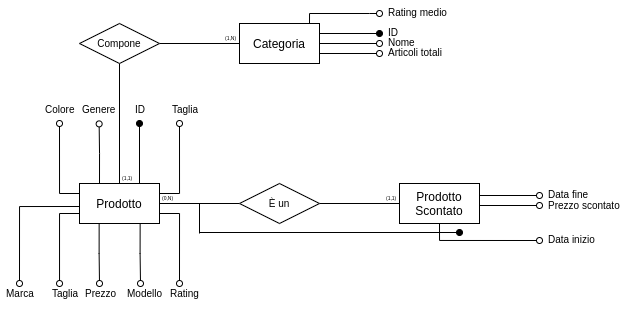
\includegraphics[scale=0.65]{images/prodotto.png}
\textbf{Le chiavi candidate nell'entità prodotto sono ID e la tupla di attributi (Modello, Marca, Taglia, Colore, Genere)}, si è scelto di utilizzare la prima come chiave primaria e rendere univoco l'insieme formato dall'altra.
\subsubsection{Segnalazione}
\begin{center}
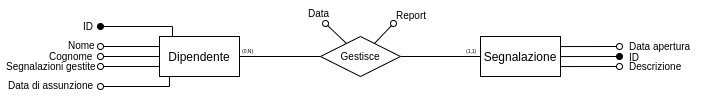
\includegraphics[scale=0.60]{images/segnalazione.png}
\end{center}
Data la relazione 1 a 1 tra Segnalazione e Rimborso \textbf{è possibile utilizzare l'ID stesso della segnalazione come chiave primaria nell'entità Rimborso}, \textbf{la stessa considerazione vale per l'entità Report}, legata a Segnalazione attraverso la relazione \textit{Associato a}.
\subsubsection{Schema finale}
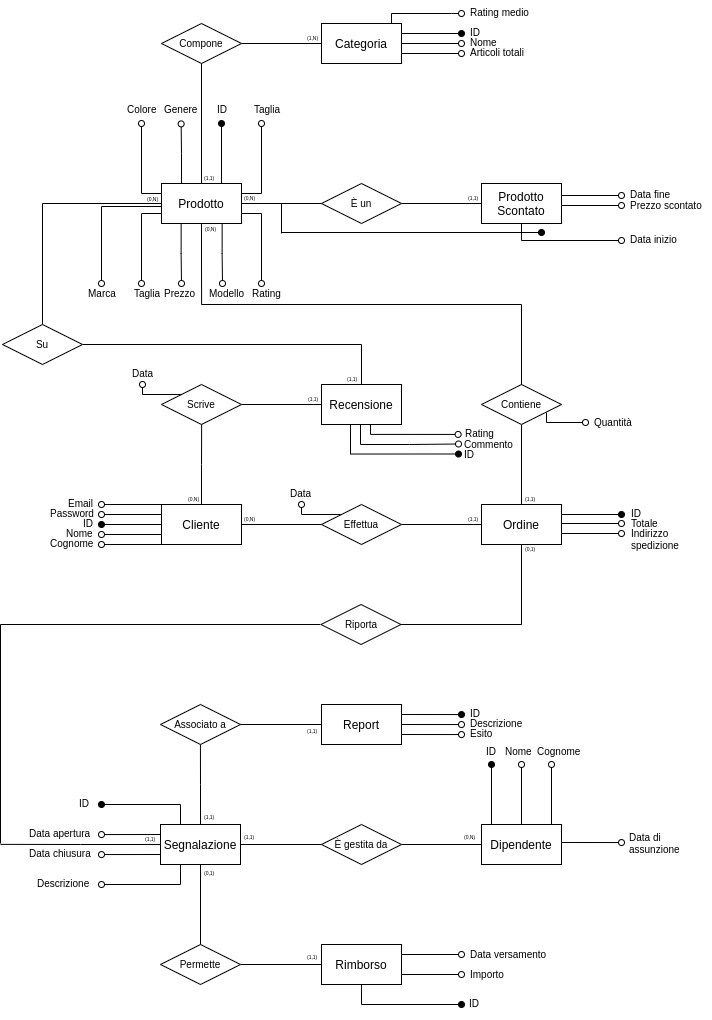
\includegraphics[scale=0.50]{images/schema_finale.png}
Le chiavi candidate dell'entità Recensione sono: ID e la coppia (ID\_cliente, ID\_prodotto), si è deciso di usare la l'\textbf{ID come chiave primaria} e\textit{ rendere univoca la coppia data dalle chiavi esterne}.
Si noti che nell'entità Segnalazione si poteva scegliere di utilizzare la chiave esterna ID\_ordine come chiave primaria, poiché legato in una relazione 1 a 1 con l'entità Ordine.